\section{Nondeterministic Finite Automaton}
(( NOTE: SHARPEN UP SECTION TO A MORE PRECISE DEFINITION OF NFA))

\begin{mydef}
An nondeterministic finite automaton (NFA) consists of a finite set of states, $Q$, with a finite number of transitions, $T$, between them.

%$T$ is a relation behavior \begin{math}\end{math}

In $Q$ there's one starting state, and a subset of accepting (final) states.

Each transition in $T$ is a has a starting state, and a destination state, and is labeled either by a character, or by $\epsilon$, which indicates an epsilon-transition (empty transition).
\end{mydef}

\subsection{Conversion from RE to NFA}
\label{RA_TO_NFA}
One of the main reasons for using NFAs when working with regular expressions is the direct correlation between regular expressions and NFAs. Each expression can be converted to an NFA, and vice versa. Table~\ref{tab:NFA_TAB} shows the correlation between regular expressions and NFA for the most common expressions.
%\\
%(( NOTE: We'll include a table with conversions ))
%\\
%With little effort every regular expression can be translated into a graph, which can then be analysed.

\begin{table}[h!]
\caption{Translation table from regular expressions to NFA}
\centering
\begin{tabular}{*{2}{m{0.4\textwidth}}}
\hline
\begin{center}$a$\end{center} &\begin{center} 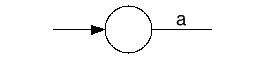
\includegraphics[width=0.25\textwidth]{lib/dot/a.png} \end{center} \\
\hline
\begin{center}$\epsilon$\end{center} &\begin{center} 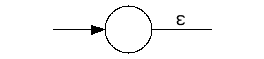
\includegraphics[width=0.25\textwidth]{lib/dot/epsilon.png} \end{center} \\
\hline
\begin{center}$ab$\end{center} &\begin{center} 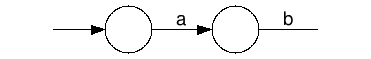
\includegraphics[width=0.3\textwidth]{lib/dot/ab.png} \end{center} \\
\hline
\begin{center}$a\vert b$\end{center} &\begin{center} 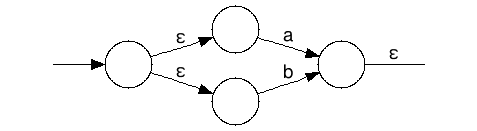
\includegraphics[width=0.35\textwidth]{lib/dot/a-or-b.png} \end{center} \\
\hline
\begin{center}$a^*$\end{center} &\begin{center} 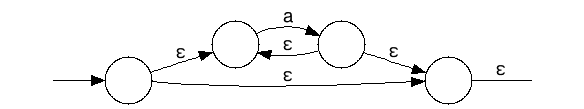
\includegraphics[width=0.4\textwidth]{lib/dot/a_star.png} \end{center} \\
\hline
\end{tabular}
\label{tab:NFA_TAB}
\end{table}

%
%\begin{figure}[h!]
 % \centering
%\begin{minipage}[b]{0.40\linewidth}
 % \centering
   %   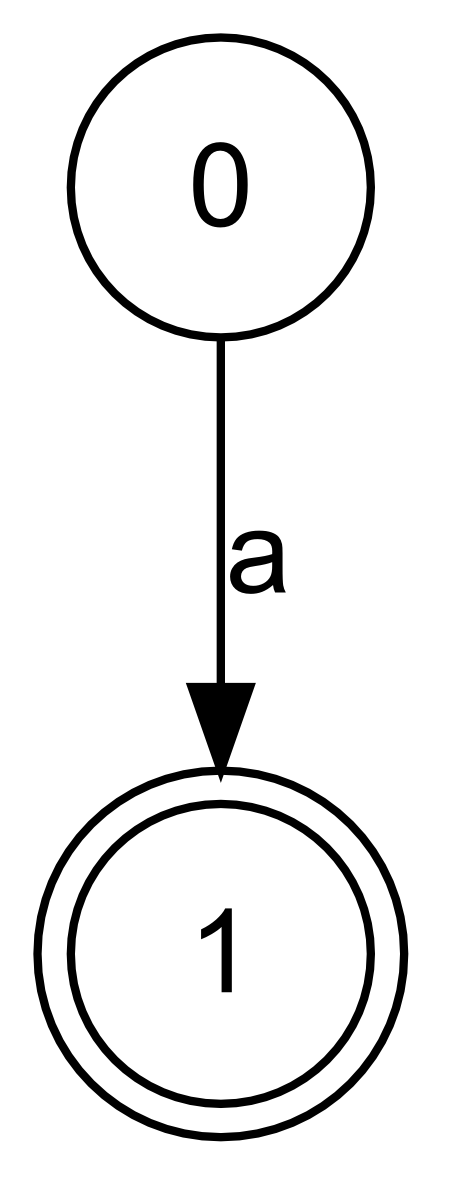
\includegraphics[width=0.2\textwidth]{lib/A.png}
  %\caption{NFA of the expression $a$}
%\label{fig:A}
%  \end{minipage}
%\begin{minipage}[b]{0.40\linewidth}

%  \centering
   %   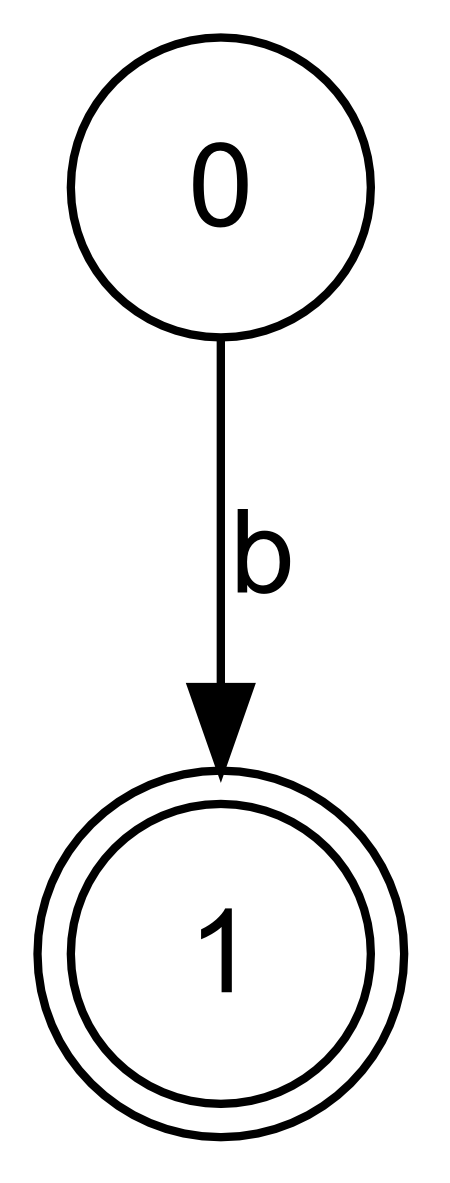
\includegraphics[width=0.2\textwidth]{lib/B.png}
  %\caption{NFA of the expression $b$}
  %\label{fig:B}
%    \end{minipage}
%\end{figure}

%For example two NFAs of regular expression $a$ and $b$ will appear as shown in Figure~\ref{fig:A} \& \ref{fig:B}, each of them starts in node $0$ and ends in node $1$, and these nodes are connected by a one-way transition with a value $a$ or $b$. %, it may be worth noting that our implementation always converts to lower case when constructing and matching.

%To construct the NFA for $A | B$ , one will first have to construct an NFA for both $A$ and $B$, which will then be combined, making the full NFA. The $|$ operator this is achieved by constructing two new nodes, the first having epsilon-transition pointing to the start node of each of the two NFAs $A$ and $B$, then for each NFA $A$ and $B$ the ending node will instead of ending the NFA, have a new epsilon-transition to the second new node, in the figure below, Figure~\ref{fig:A_OR_B}, the two new nodes are labeled $0$ and $5$:

%\begin{figure}[h!]
 % \centering
   %   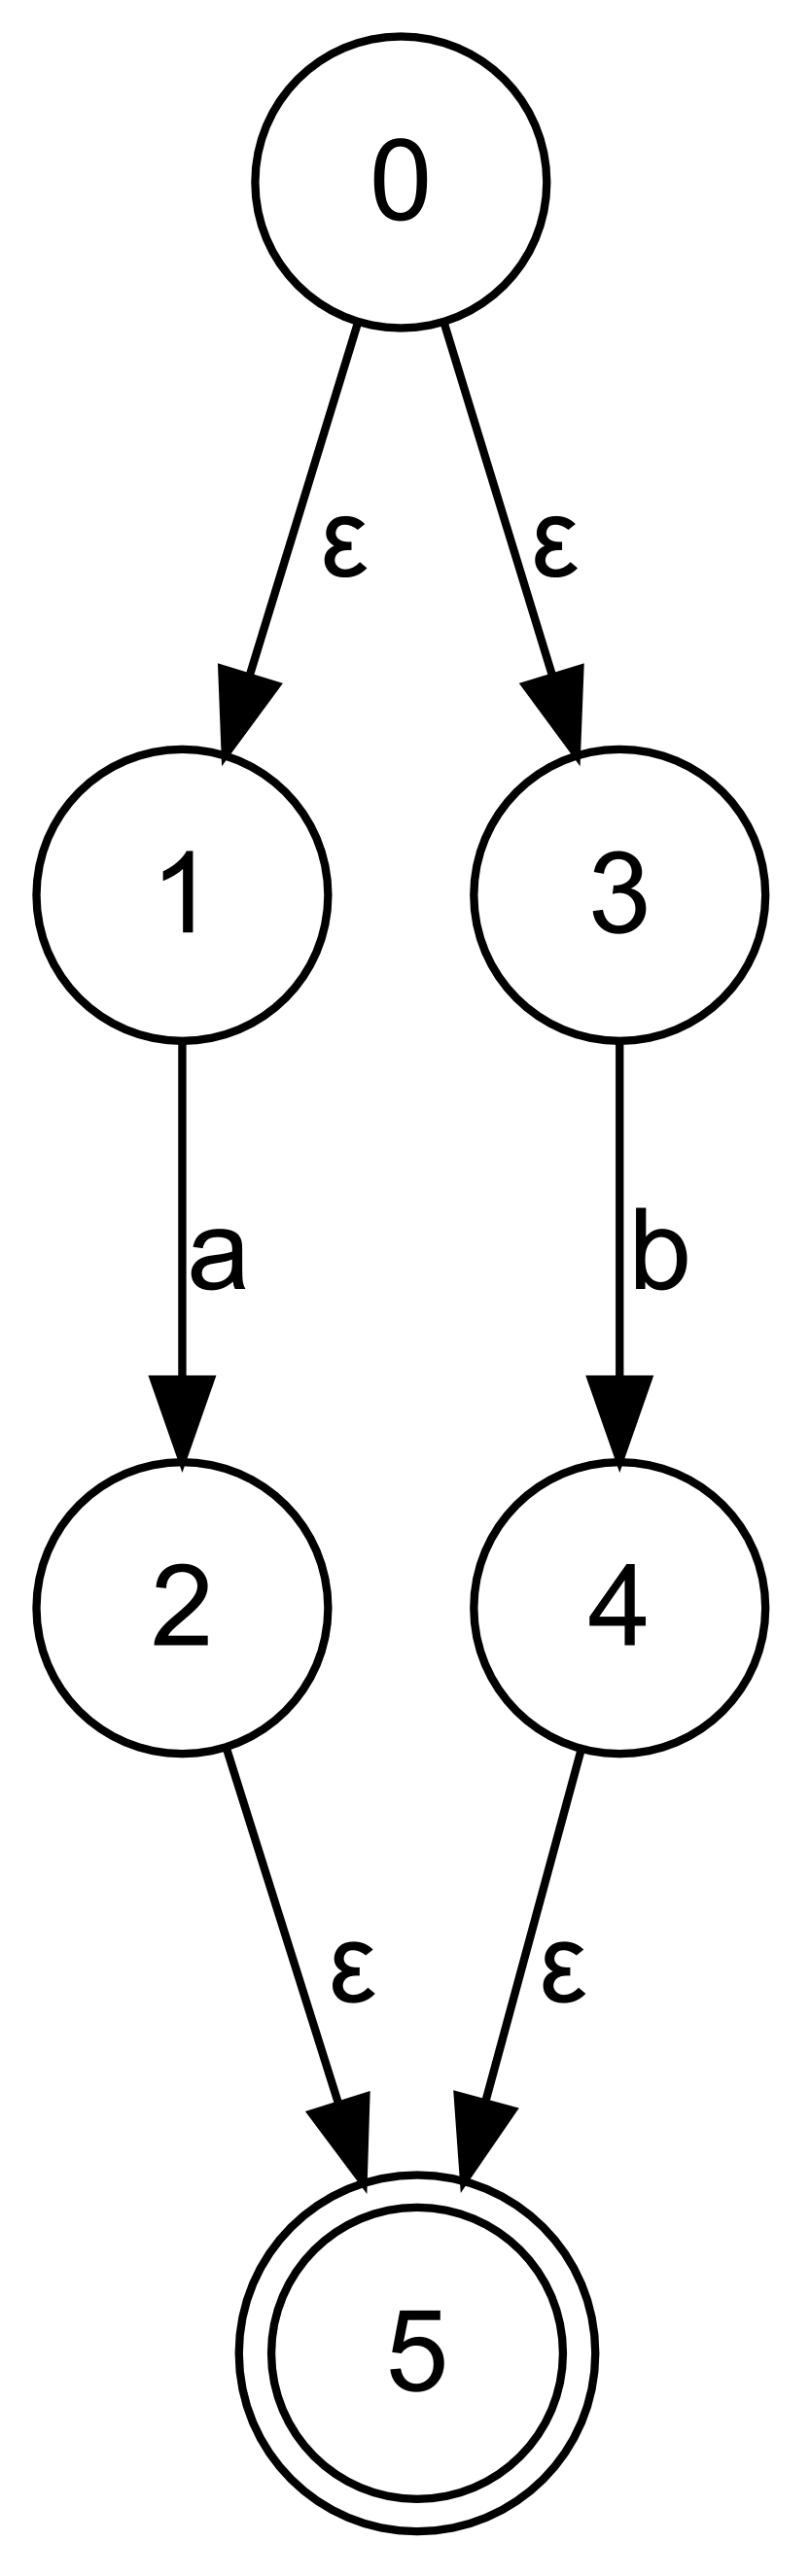
\includegraphics[width=0.1\textwidth]{lib/A_OR_B.png}
 % \caption{NFA of the expression $a | b$}
%\label{fig:A_OR_B}
%\end{figure}

Once a NFA-structure has been build, we can start matching a text against the NFA.

This is achieved by having a set of states, each state is looking at a node in the structure, while keeping track of previous nodes traversed by the state. Whenever a new character is being checked to match, each state will look at its node, and determine if it's possible to accept the character in the NFA, either by taking a transition labeled with the character, or alternatively via an epsilon-transition. When two possible transitions are viable, new states will be created in the set of states, so that each possible transition will be explored.

Any state that will fail to match the character will be removed from the set of states.
%\begin{figure}[h!]
 % \centering
%\begin{minipage}[b]{0.40\linewidth}
 % \centering
   %   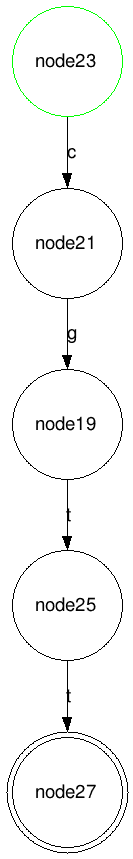
\includegraphics[width=0.2\textwidth]{lib/cgtt1.png}
   % \caption{NFA of $CGTT$, with a state looking at node23.\\}
    %\label{fig:CGTT_1}
 % \end{minipage}
%\begin{minipage}[b]{0.40\linewidth}
%\centering
%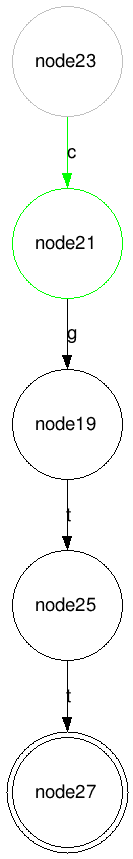
\includegraphics[width=0.2\textwidth]{lib/cgtt2.png}
% \caption{Next iteration of the state on Figure~\ref{fig:CGTT_1}, the state is now in node21.}
  %  \end{minipage}
%\label{fig::cgtt}
%\end{figure}

Only if a state reaches the ending node of the NFA, there's a match.

\newpage

\subsection{Insertions, Deletions and Mutations}
NFAs do not support mismatching by default, although a regular expression can be built to handle mismatches. While doing handling mismatching while constructing the regular expression, we are interested in having an NFA, and allowing matching while with support for insertions, deletions and mutations, hence we need to define a way to handle this.

We can do this by adding a counter for insertions, deletions and mutations, and when a transition is not possible in the NFA, we decrease these counters and preform alternative transitions to emulate these conditions.
%Currently our implementation supports a simple solution to the insertion, deletion and mutation problem, which is achieved by having a counter for insertions, deletions and mutation in each state, these counters symbolise the number of allowed occurrences of each mutation, insertion and deletion.
\begin{description}
\item[] For insertions, the state will remember the unmatched character, but the state won't move from its current node.
\item[]For deletions, the state wont remember the unmatched character, but it will take every transition going on from the node.
\item[] For mutations, the same happens as in a deletion, but now the state also remembers the unmatched character.
\end{description}
Figure~\ref{fig:ins_mut_del} illustrates how states move through a NFA when mismatches occur. 

\begin{figure}[h!]
  \centering
      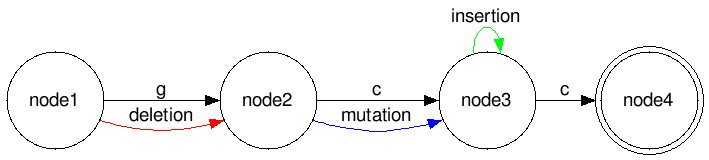
\includegraphics[width=0.6\textwidth]{lib/gcc_ins_mut_del.png}
  \caption{Simple NFA of $GCC$, showing behaviour of insertion, mutation and deletion}
\label{fig:ins_mut_del}
\end{figure}
%Depending on the number of insertions, deletions and mutations allowed, this approach will grant each state a much longer lifespan, and for each non-matching character parsed, one state may turn into three, which all needs to be processed for each new character parsed, resulting in an increasingly slower running time as the allowed number of insertions, deletions and mutations increase, but it does give us the utility that we require.
%\label{state:insertion1}


%In the next iteration of our implementation, we aim to implement levenstein automations\cite{WikiLevenshtein}, which hopefully will help speed up the runtime, and also, currently our solution will work on any given regular expression, thus a logical step which also may deliver some increase in performance would be to enforce a constriction such that it only allows for a RNA language similar to that defined in Section~\ref{section:RE}.